\section{Uppgift 2}\label{uppgift-2}

\subsection{Instruktioner}
\begin{verbatim}
2. Skriv ett program som skriver ut summan, medelvärdet och produkten av tre
   heltal.  De tre heltalen ska användaren skriva in från tangentbordet när
   programmet körs. Programmets utskrift kan t.ex se ut så här, det som skrivs
   in från tangentbordet är markerat med fetstil/understrykning:

    Skriv in tre heltal.
    Skriv in det första talet: *20*
    Skriv in det andra talet: *30*
    Skriv in det tredje talet: *25*
    Summan av talen är 75.
    Medelvärdet av talen är 25.
    Produkten av talen är 15000.
\end{verbatim}

\subsection{Lösning}
\subsubsection{Funktion}
Programmet använder \texttt{static final} i början av programmet för variabler
som inte ska ändras under exekvering.  Variabler med enbart versaler är en
slags globala variabler som kan modifieras av programmeraren.
\par Räkneord sparas i sträng-arrays \texttt{GRUNDTAL} och
\texttt{ORDNINGSTAL}, för att hämtas och skrivas ut vid exekvering.

\subsubsection{Kommentar}
\par Rad 33, \texttt{@SuppressWarnings("resource")} syftar till att undertrycka
varningar från Eclipse och gör ingen faktisk skillnad på programmets funktion.
\par Programmet saknar filtrering av indata, vilket är ett stort problem då det
innebär stora säkerhetsrisker och möjliga odefinerade, alternativt outforskade
skeenden. Mer om detta senare..

\subsubsection{Källkod}\label{uppgift-2_src}
%\begin{listing}[H]
    \inputminted[linenos]{java}{src/Lab1Uppg02.java}
    \caption{Lab1Uppg02.java}
    \label{Uppg2src}
%\end{listing}

\subsubsection{Skärmdump}
\begin{figure}[htbp]
    \centering
        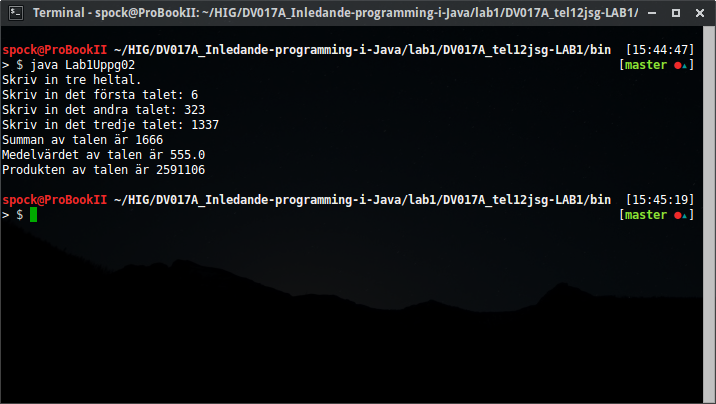
\includegraphics[width=\linewidth]{img/02.png}
    \caption{Körning av koden till Uppgift \ref{uppgift-2}}
    \label{fig:screenshot-02}
\end{figure}
